% Standalone wrapper for the signal-conversion figure.
%
%   py -3.12 paper/figures/build_signal_conversion_figure.py
%
% Produces fig_signal_conversion.pdf next to this file.  The main document
% (paper/main.tex) includes that PDF, so the figure is always available.
%
% mathptmx/times provides the same Times metrics that IEEEtran uses for the
% main text, so the standalone PDF is typographically identical to the
% in-document rendering (same glyph widths -> no unexpected line breaks).
% border=0 + varwidth/varheight: the page is cut to exactly the IEEEtran text
% width (18.13 cm) and to the height of the drawing, so the document can
% include the PDF with width=\textwidth and obtain a scale of 1.000; the
% declared point sizes are then the printed sizes.
\documentclass[border=0pt,varwidth=18.13cm,varheight=6.15cm]{standalone}
\usepackage[T1]{fontenc}
\usepackage{times}
\usepackage{amsmath,amssymb}
\usepackage{xcolor}
\usepackage{tikz}
\usetikzlibrary{positioning}
% NOTE: \parboxsep is not defined by every LaTeX kernel (the Tectonic bundle
% used here does not provide it), and PGF's \parbox-based text boxes do not
% use it either -- the node width is text width + 2 * inner sep.  The figure
% therefore relies on inner sep only and must not set \parboxsep.
\begin{document}
% ---------------------------------------------------------------------------
% fig_signal_conversion.tex
%
% Signal-level view of the transformation performed by A2L-RAGAlign.
% Reading order (one pipeline, not two):
%   (1) numbered stage headers 1-7  -- the conversion pipeline
%   (2) three table rows            -- one concrete trace per stage
%   (3) lower band 4a-4f            -- internals of stage 4, called out
%       by an orthogonal dashed bracket from column 4 (not a second
%       independent flowchart)
%
% Every identifier, address, data type, object kind and score shown here is
% reproducible from the artifacts shipped with the tool:
%   data/sample/example.map            demonstration address file (16 symbols)
%   data/sample/example_updated.a2l    regenerated description
%   rag_align.py + A2L_Update_Tool_main.py (ALL_SIGNALS): the 83-document
%                                    embedded knowledge base and the aligner
%   scores: SemanticAligner(kb, tau_auto=0.45, tau_suggest=0.30), two
%            scoring channels (2/3 retrieval, 1/3 token); the structural
%            evidence is an input of the contract check, not a score term
%   class-flip twin: meas_EngineSpeed_C -> Eng_Speed_u16_M, 0.5535 before and
%                    0.3044 after the 0.55 penalty (hard cap, SUGGEST)
%
% ASCII-only on purpose: the paper is built with pdfLaTeX (no CJK support).
%
% ---------------------------------------------------------------------------
% TYPOGRAPHY (IEEE style)
%   The figure uses the same type family as the body text: the Times
%   (Nimbus Roman) text of IEEEtran, the Courier typewriter that IEEEtran
%   selects for identifiers, and the Computer Modern math of the paper.
%   Two type sizes are used -- no more, so that the figure reads as one
%   typographic system:
%       l1 = 8 pt  structural labels  (zone captions, stage headers)
%       l2 = 6 pt  data content      (table cells, lower band, annotations)
%   Bold is used only for the leading keyword of a cell or a box, the
%   typewriter face is used for every identifier, A2L keyword, tool and
%   file-format name (AXF/ELF, DWARF, MEASUREMENT, INCA), and italic is
%   reserved for the zone captions.  The picture is 18.13 cm wide, i.e. the
%   IEEEtran text width (7.14 in); the document includes it with
%   width=0.80\textwidth, so the printed sizes are 0.80 x the point sizes
%   above (8 pt -> 6.4 pt, 6 pt -> 4.8 pt).  The 6 pt style is used for the
%   bulk text and the 5 pt style only for single-letter sub-labels of the
%   fusion weights, so the smallest printed glyph is a fraction numerator
%   rather than a readable word.  Widening the inclusion beyond 0.80 costs
%   two full lines of body text per 0.05, because this is a figure* and the
%   height is charged to both columns.
%
% STAGE HEADERS (one rule, applied to all seven columns)
%   The number and the keyword of a stage are bold; the explanatory lines
%   below are roman.  A header never ends on a dangling operator: a sign
%   that continues into the next line ("Identity +") is written out in
%   words instead ("Identity / metadata"), and two parallel items
%   are separated by a slash, as in the object and bench columns
%   ("MEASUREMENT / CHARACTERISTIC", "INCA / CANape").  The plus sign is
%   reserved for combining two sources ("AXF/ELF + DWARF").
%
% THRESHOLDS
%   The tier thresholds are written $\tau_{\mathrm{a}}$ (AUTO) and
%   $\tau_{\mathrm{s}}$ (SUGGEST), i.e. exactly the symbols used in the text;
%   the code calls them tau_auto and tau_suggest.  The short form is forced
%   by the width of column 5 (1.48 cm), which cannot hold the long names.
%
% COLOUR (one meaning per colour, so no legend is needed)
%   black / grey  the deterministic base tool, the rules, the annotations
%   blue         the retrieval-augmented layer (stage 4, the lower band and
%                 the names it retrieves)
%   green AUTO   orange SUGGEST   red MANUAL and the hard-capped branch
%
% GEOMETRY (all lengths in cm; a strict grid, so the result is aligned line
% by line).  Every column width is derived from the measured natural width
% of its longest entry (\sbox harness in _measure8.tex, then calibrated
% against the rendered line widths of the final PDF), so no cell can wrap
% and no entry can collide with a column rule.
%   table width      0.00 .. 18.13
%   column rules     0.80 | 3.80 | 6.32 | 7.98 | 11.53 | 13.01 | 15.93
%                    (row label, then stages 1..7)
%   column widths    0.80 | 3.00 | 2.52 | 1.66 | 3.55 | 1.48 | 2.92 | 2.20
%   cell padding     0.07 on the left and on the right of every column
%   header boxes     inset 0.11 on both sides of their column, all 1.14 cm
%                    high, so the header row is aligned as well
%   table rules      y = -1.68 | -2.36 | -3.04 | -3.72
%   table cells      top aligned 0.075 below their rule, so that the first
%                    line of all cells of a row shares one baseline
%   lower band       six equal boxes (outer 2.771, gap 0.30) spanning exactly
%                    the table width, centres 1.386 | 4.457 | 7.529 |
%                    10.601 | 13.672 | 16.744; numbered 4a-4f because they
%                    are the internals of stage 4, not a second pipeline
%   stage-4 callout  orthogonal dashed bracket from the two bottom corners
%                    of column 4 (x = 7.98 and 11.53, y = -3.72) down to
%                    y = -4.24, then out to the band corners (x = 0.02 and
%                    18.11) and down into the band at y = -4.44
%   rejected branch  box width identical to the box it hangs from
%
%   Every multi-line node ends each of its lines with \fsstrut.  The strut
%   fixes the height and the depth of every line, so all lines of a row or
%   of a box share one baseline grid and all boxes of a band have the same
%   height -- that is what makes the drawing look aligned.
% ---------------------------------------------------------------------------
\providecommand{\fsstrut}{\strut}
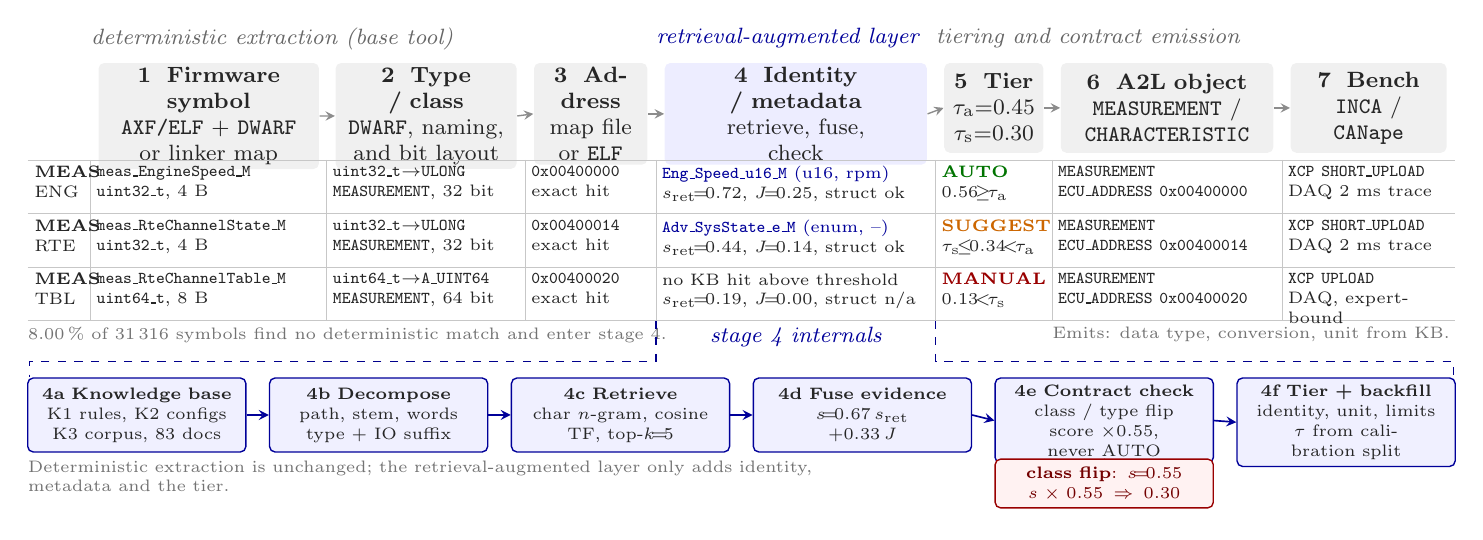
\begin{tikzpicture}[
    >=stealth,
    every node/.style={align=center},
    % ---- IEEE type scale: two sizes only -----------------------------------
    l1/.style={font=\fontsize{8}{9.4}\selectfont},
    l2/.style={font=\fontsize{6}{7.2}\selectfont},
    % ---- stage headers ----------------------------------------------------
    hd/.style={l1, draw=none, fill=black!6, text=black!85,
              minimum height=1.14cm, inner sep=1.5pt, rounded corners=2pt,
              line width=0.5pt, align=center},
    hdr/.style={hd, fill=blue!7},
    % ---- table cells ------------------------------------------------------
    cel/.style={l2, text=black!85, inner sep=0pt, align=left,
                anchor=north west},
    % ---- lower band -------------------------------------------------------
    rb/.style={l2, draw=blue!60!black, fill=blue!6, text=black!85,
               text width=2.595cm, minimum height=0.94cm, inner sep=2.5pt,
               rounded corners=2pt, line width=0.5pt, align=center},
    rr/.style={l2, draw=red!60!black, fill=red!5, text=red!45!black,
               text width=2.665cm, minimum height=0.62cm, inner sep=1.5pt,
               rounded corners=2pt, line width=0.5pt, align=center},
    % ---- lines ------------------------------------------------------------
    fl/.style={->, line width=0.5pt, draw=black!45},
    flb/.style={->, line width=0.6pt, draw=blue!60!black},
    flr/.style={->, dashed, line width=0.6pt, draw=red!60!black},
    rule/.style={line width=0.3pt, draw=black!22},
    cone/.style={dashed, line width=0.5pt, draw=blue!55!black},
    % ---- captions and notes ----------------------------------------------
    zl/.style={l1, font=\fontsize{8}{9.4}\selectfont\itshape, text=black!60,
               anchor=north west, inner sep=0pt},
    zlb/.style={zl, text=blue!60!black},
    note/.style={l2, text=black!55, align=left, inner sep=0pt},
]
% ====================== zone captions (top) ==============================
\node[zl,  anchor=north west] at (0.80,0.00)
    {deterministic extraction (base tool)};
\node[zlb, anchor=north west] at (7.98,0.00)
    {retrieval-augmented layer};
\node[zl,  anchor=north west] at (11.53,0.00)
    {tiering and contract emission};

% ====================== stage headers ===================================
\node[hd,  anchor=north, text width=2.694cm] (h1) at (2.300,-0.44)
    {\textbf{1~~Firmware symbol}\fsstrut\\
     \texttt{AXF/ELF} + \texttt{DWARF}\fsstrut\\
     or linker map\fsstrut};
\node[hd,  anchor=north, text width=2.194cm] (h2) at (5.060,-0.44)
    {\textbf{2~~Type / class}\fsstrut\\
     \texttt{DWARF}, naming,\fsstrut\\
     and bit layout\fsstrut};
\node[hd,  anchor=north, text width=1.334cm] (h3) at (7.150,-0.44)
    {\textbf{3~~Address}\fsstrut\\
     map file\fsstrut\\
     or \texttt{ELF}\fsstrut};
\node[hdr, anchor=north, text width=3.224cm] (h4) at (9.755,-0.44)
    {\textbf{4~~Identity / metadata}\fsstrut\\
     retrieve, fuse,\fsstrut\\
     check\fsstrut};
\node[hd,  anchor=north, text width=1.154cm] (h5) at (12.270,-0.44)
    {\textbf{5~~Tier}\fsstrut\\
     $\tau_{\mathrm{a}}{=}0.45$\fsstrut\\
     $\tau_{\mathrm{s}}{=}0.30$\fsstrut};
\node[hd,  anchor=north, text width=2.594cm] (h6) at (14.470,-0.44)
    {\textbf{6~~A2L object}\fsstrut\\
     \texttt{MEASUREMENT} /\fsstrut\\
     \texttt{CHARACTERISTIC}\fsstrut};
\node[hd,  anchor=north, text width=1.874cm] (h7) at (17.030,-0.44)
    {\textbf{7~~Bench}\fsstrut\\
     \texttt{INCA} /\fsstrut\\
     \texttt{CANape}\fsstrut};
\foreach \a/\b in {h1/h2,h2/h3,h3/h4,h4/h5,h5/h6,h6/h7} {
    \draw[fl] (\a.east) -- (\b.west);
}

% ====================== table rules =====================================
\draw[rule] (0,-1.68) -- (18.13,-1.68);
\draw[rule] (0,-2.36) -- (18.13,-2.36);
\draw[rule] (0,-3.04) -- (18.13,-3.04);
\draw[rule] (0,-3.72) -- (18.13,-3.72);
\foreach \x in {0.80,3.80,6.32,7.98,11.53,13.01,15.93} {
    \draw[rule] (\x,-1.68) -- (\x,-3.72);
}
% ====================== row 1: measured engine speed ====================
\node[cel, text width=0.66cm] at (0.08,-1.755)
    {\textbf{MEAS}\fsstrut\\ENG\fsstrut};
\node[cel, text width=2.86cm] at (0.87,-1.755)
    {\texttt{meas\_EngineSpeed\_M}\fsstrut\\
     \texttt{uint32\_t}, 4 B\fsstrut};
\node[cel, text width=2.38cm] at (3.87,-1.755)
    {\texttt{uint32\_t}$\rightarrow$\texttt{ULONG}\fsstrut\\
     \texttt{MEASUREMENT}, 32 bit\fsstrut};
\node[cel, text width=1.52cm] at (6.39,-1.755)
    {\texttt{0x00400000}\fsstrut\\exact hit\fsstrut};
\node[cel, text width=3.41cm] at (8.05,-1.755)
    {\textcolor{blue!60!black}{\texttt{Eng\_Speed\_u16\_M} (u16, rpm)}\fsstrut\\
     $s_{\mathrm{ret}}\!{=}\!0.72$, $J\!{=}\!0.25$, struct ok\fsstrut};
\node[cel, text width=1.34cm] at (11.60,-1.755)
    {\textbf{\textcolor{green!45!black}{AUTO}}\fsstrut\\$0.56\!{\geq}\!\tau_{\mathrm{a}}$\fsstrut};
\node[cel, text width=2.78cm] at (13.08,-1.755)
    {\texttt{MEASUREMENT}\fsstrut\\
     \texttt{ECU\_ADDRESS} \texttt{0x00400000}\fsstrut};
\node[cel, text width=2.06cm] at (16.00,-1.755)
    {\texttt{XCP SHORT\_UPLOAD}\fsstrut\\DAQ 2 ms trace\fsstrut};
% ====================== row 2: RTE channel state =========================
\node[cel, text width=0.66cm] at (0.08,-2.435)
    {\textbf{MEAS}\fsstrut\\RTE\fsstrut};
\node[cel, text width=2.86cm] at (0.87,-2.435)
    {\texttt{meas\_RteChannelState\_M}\fsstrut\\
     \texttt{uint32\_t}, 4 B\fsstrut};
\node[cel, text width=2.38cm] at (3.87,-2.435)
    {\texttt{uint32\_t}$\rightarrow$\texttt{ULONG}\fsstrut\\
     \texttt{MEASUREMENT}, 32 bit\fsstrut};
\node[cel, text width=1.52cm] at (6.39,-2.435)
    {\texttt{0x00400014}\fsstrut\\exact hit\fsstrut};
\node[cel, text width=3.41cm] at (8.05,-2.435)
    {\textcolor{blue!60!black}{\texttt{Adv\_SysState\_e\_M} (enum, --)}\fsstrut\\
     $s_{\mathrm{ret}}\!{=}\!0.44$, $J\!{=}\!0.14$, struct ok\fsstrut};
\node[cel, text width=1.34cm] at (11.60,-2.435)
    {\textbf{\textcolor{orange!80!black}{SUGGEST}}\fsstrut\\$\tau_{\mathrm{s}}\!{\leq}\!0.34\!{<}\!\tau_{\mathrm{a}}$\fsstrut};
\node[cel, text width=2.78cm] at (13.08,-2.435)
    {\texttt{MEASUREMENT}\fsstrut\\
     \texttt{ECU\_ADDRESS} \texttt{0x00400014}\fsstrut};
\node[cel, text width=2.06cm] at (16.00,-2.435)
    {\texttt{XCP SHORT\_UPLOAD}\fsstrut\\DAQ 2 ms trace\fsstrut};
% ====================== row 3: uncovered RTE table =======================
\node[cel, text width=0.66cm] at (0.08,-3.115)
    {\textbf{MEAS}\fsstrut\\TBL\fsstrut};
\node[cel, text width=2.86cm] at (0.87,-3.115)
    {\texttt{meas\_RteChannelTable\_M}\fsstrut\\
     \texttt{uint64\_t}, 8 B\fsstrut};
\node[cel, text width=2.38cm] at (3.87,-3.115)
    {\texttt{uint64\_t}$\rightarrow$\texttt{A\_UINT64}\fsstrut\\
     \texttt{MEASUREMENT}, 64 bit\fsstrut};
\node[cel, text width=1.52cm] at (6.39,-3.115)
    {\texttt{0x00400020}\fsstrut\\exact hit\fsstrut};
\node[cel, text width=3.41cm] at (8.05,-3.115)
    {no KB hit above threshold\fsstrut\\
     $s_{\mathrm{ret}}\!{=}\!0.19$, $J\!{=}\!0.00$, struct n/a\fsstrut};
\node[cel, text width=1.34cm] at (11.60,-3.115)
    {\textbf{\textcolor{red!60!black}{MANUAL}}\fsstrut\\$0.13\!{<}\!\tau_{\mathrm{s}}$\fsstrut};
\node[cel, text width=2.78cm] at (13.08,-3.115)
    {\texttt{MEASUREMENT}\fsstrut\\
     \texttt{ECU\_ADDRESS} \texttt{0x00400020}\fsstrut};
\node[cel, text width=2.06cm] at (16.00,-3.115)
    {\texttt{XCP UPLOAD}\fsstrut\\DAQ, expert-bound\fsstrut};
% ====================== notes + orthogonal callout of stage 4 ===========
% The dashed polyline is a 90-degree exploded-view bracket: column 4 of
% the table is stage 4, and the lower band is that stage opened up
% (4a-4f).  No arrowheads -- this is a callout, not a data-flow.
\node[note, anchor=north west] at (0.00,-3.80)
    {8.00\,\% of 31\,316 symbols find no deterministic match and enter stage 4.\fsstrut};
\draw[cone] (7.98,-3.72) -- (7.98,-4.24) -- (0.02,-4.24) -- (0.02,-4.44);
\draw[cone] (11.53,-3.72) -- (11.53,-4.24) -- (18.11,-4.24) -- (18.11,-4.44);
\node[zlb, anchor=north] at (9.755,-3.80)
    {stage 4 internals};
\node[note, anchor=north west] at (13.01,-3.80)
    {Emits: data type, conversion, unit from KB.\fsstrut};

% ====================== lower band: retrieval-augmented layer ============
\node[rb, anchor=north] (b0) at (1.386,-4.44)
    {\textbf{4a~Knowledge base}\fsstrut\\
     K1 rules, K2 configs\fsstrut\\
     K3 corpus, 83 docs\fsstrut};
\node[rb, anchor=north] (b1) at (4.457,-4.44)
    {\textbf{4b~Decompose}\fsstrut\\
     path, stem, words\fsstrut\\
     type + IO suffix\fsstrut};
\node[rb, anchor=north] (b2) at (7.529,-4.44)
    {\textbf{4c~Retrieve}\fsstrut\\
     char $n$-gram, cosine\fsstrut\\
     TF, top-$k\!{=}\!5$\fsstrut};
\node[rb, anchor=north] (b3) at (10.601,-4.44)
    {\textbf{4d~Fuse evidence}\fsstrut\\
     $s\!{=}\!0.67\,s_{\mathrm{ret}}$\fsstrut\\
     ${+}0.33\,J$\fsstrut};
\node[rb, anchor=north] (b4) at (13.672,-4.44)
    {\textbf{4e~Contract check}\fsstrut\\
     class / type flip\fsstrut\\
     score $\times 0.55$, never AUTO\fsstrut};
\node[rb, anchor=north] (b5) at (16.744,-4.44)
    {\textbf{4f~Tier + backfill}\fsstrut\\
     identity, unit, limits\fsstrut\\
     $\tau$ from calibration split\fsstrut};
\foreach \a/\b in {b0/b1,b1/b2,b2/b3,b3/b4,b4/b5} {
    \draw[flb] (\a.east) -- (\b.west);
}

% ====================== rejected branch: class-flip twin =================
\draw[flr] (b4.south) -- (13.672,-5.47);
\node[rr, anchor=north, inner sep=1.5pt] at (13.672,-5.47)
    {\textbf{class flip}: $s\!{=}\!0.55$\fsstrut\\
     $s \times 0.55 \Rightarrow 0.30$\fsstrut};

% ====================== closing note ====================================
\node[note, anchor=north west, text width=10.00cm] at (0.00,-5.49)
    {Deterministic extraction is unchanged; the retrieval-augmented layer
     only adds identity, metadata and the tier.\fsstrut};
% The picture is pinned to the exact IEEEtran text width (18.13 cm) and to
% its own height (6.15 cm); the standalone wrapper cuts the page to the
% same box, so the document can include the PDF with width=\textwidth and
% obtain a scale of 1.000.
\pgfresetboundingbox
\path[use as bounding box] (0,0) rectangle (18.13,-6.15);
\end{tikzpicture}%
%
\end{document}
